\documentclass[ignorenonframetext,t]{beamer}
%\usetheme{2ndQuadrantTraining}

\usepackage[spanish]{babel}
\usepackage[T1]{fontenc}
\usepackage[utf8]{inputenc}
% 19.5x9 is alvherre's current phone aspect ratio
\geometry{papersize={19.5cm,9cm}}
\IfFileExists{upquote.sty}{\usepackage{upquote}}{}

\institute{2ndQuadrant -- Professional PostgreSQL}
\date{Valdivia, Chile, Agosto 2020}

\usepackage{pmboxdraw}

\usepackage{listings}
\lstset{language=SQL,
basicstyle=\footnotesize\ttfamily,keywordstyle=\bfseries, columns=fullflexible, upquote,
showspaces=false,showstringspaces=false,
literate={á}{{\'{a}}}{1}
         {é}{{\'{e}}}{1}
         {í}{{\'{i}}}{1}
         {ó}{{\'{o}}}{1}
         {ú}{{\'{u}}}{1}
         {¡}{{!`}}{1}
         {┌}{{\textSFi}}1 
         {─}{{\textSFx}}1 
         {│}{{\pmboxdrawuni{2502}}}1
         {┬}{{\textSFvi}}1
         {┐}{{\textSFiii}}1
         {├}{{\textSFviii}}1
         {┼}{{\textSFv}}1
         {┤}{{\textSFix}}1
         {┴}{{\textSFvii}}1
         {└}{{\textSFii}}1
         {┘}{{\textSFiv}}1
%morekeywords={data,wrapper,library,language}%
}

\title{PostgreSQL: La Ruta del Particionamiento}
\newcommand{\putcollection}{
  \put(0,50){
    \parbox{\textwidth}{
      \fontsize{30}{30}\selectfont
      Álvaro Herrera \\
      PostgreSQL developer \\
      2ndQuadrant Ltd., Valdivia, Chile
    }
  }
}
\newcommand{\insertcopyright}{}
\renewcommand{\insertcopyright}{(C) 2ndQuadrant Limited 2008-2020}
%\date{}

% Make pauses show greyed-out future text
\setbeamercovered{transparent}

\begin{document}

  \begin{frame}[plain]
    \titlepage
  \end{frame}

\begin{frame}
	\frametitle{Particionamiento declarativo}

	\center 
\includegraphics{are_we_there_yet_1.jpg}

\end{frame}

\begin{frame}

	\frametitle{Particionamiento declarativo}

	\begin{itemize}
		\item Introducido en PostgreSQL 10 (2017)
		\item Mejoras significativas con cada nueva versión
		\item Más práctico de manejar para usuarios que el sistema antiguo
		\item Mejor rendimiento que el sistema antiguo en muchas áreas
			\pause
		\item ... pero aún nos faltan cosas importantes
	\end{itemize}
\end{frame}

\begin{frame}[fragile]
	\setbeamercovered{transparent}
%	\beamerdefaultoverlayspecification{<+>}
	\frametitle{DDL básico de particionamiento}
\begin{lstlisting}
CREATE TABLE pedidos (
    pedido_id BIGINT,
    pedido_fecha TIMESTAMP WITH TIME ZONE, ...
) PARTITION BY RANGE (pedido_fecha);
	\end{lstlisting}
% la tabla particionada no sabe aún cuántas particiones habrá
% ni los rangos de valores
\end{frame}

\begin{frame}
    \frametitle{Estrategias de particionamiento}

\begin{description}
	\item{\texttt{RANGE}} Rango de valores para cada columna de particionamiento
	    \vskip 1cm

	\item{\texttt{LIST}} Lista de valores para cada columna de particionamiento
	    \vskip 1cm
\pause
	\item{\texttt{HASH}} \textit{Hash} de los valores de las columnas de particionamiento
	\begin{itemize} \item Añadido en PostgreSQL 11\end{itemize}
\end{description}
\end{frame}

\begin{frame}[fragile]
	\frametitle{Estrategias de particionamiento: \texttt{RANGE}}
\begin{lstlisting}
-- crea partición vacía
CREATE TABLE pedidos_2018_01
   PARTITION OF pedidos FOR VALUES FROM ('2018-01-01') TO ('2018-02-01');
\end{lstlisting}
% cada partición tiene nombre, se puede leer directamente.
% En cada partición definimos el rango.
% Requiere AccessExclusiveLock en tabla padre
\pause
\begin{lstlisting}
-- agrega como partición una tabla existente que puede tener datos
ALTER TABLE pedidos ATTACH PARTITION pedidos_2018_02
FOR VALUES FROM ('2018-02-01') TO ('2018-03-01');
\end{lstlisting}
\pause
\begin{itemize}
	\item Intervalo cerrado a la izquierda, abierto a la derecha
\end{itemize}

\pause
\begin{itemize}
	\item ¡No se necesita trigger/regla para rutear tuplas!
	\begin{itemize} \item gran ventaja comparado con sistema antiguo \end{itemize}
\end{itemize}
% Sólo usa ShareUpdateExclusiveLock en tabla padre
\end{frame}

\begin{frame}[fragile]
	\frametitle{Estrategias de particionamiento: \texttt{RANGE} (2)}
\begin{lstlisting}
CREATE TABLE lecturas_sensores (sensor_id BIGINT, momento TIMESTAMPTZ,
     lectura DOUBLE PRECISION)
  PARTITION BY RANGE (momento, sensor_id);
\end{lstlisting}
\pause
\begin{lstlisting}
CREATE TABLE lecturas_sensores_2016 PARTITION OF lecturas_sensores
	FOR VALUES FROM ('2016-01-01', MINVALUE) TO ('2017-01-01', MINVALUE);
\end{lstlisting}
\pause
\begin{lstlisting}
CREATE TABLE lecturas_sensores_2017_1 PARTITION OF lecturas_sensores
    FOR VALUES FROM ('2017-01-01', MINVALUE) TO ('2017-01-02', 10000);
\end{lstlisting}
\pause
\begin{lstlisting}
CREATE TABLE lecturas_sensores_2017_2 PARTITION OF lecturas_sensores
	FOR VALUES FROM ('2017-07-02', MINVALUE) TO ('2018-01-01', MINVALUE);
\end{lstlisting}

\end{frame}

\begin{frame}[fragile]
	\frametitle{Estrategias de particionamiento: \texttt{LIST}}
\begin{lstlisting}
CREATE TYPE paises AS ENUM ('Argentina', 'Bolivia', 'Brasil', 'Chile', 'Colombia',
       'Costa Rica', 'Cuba', 'Ecuador', 'El Salvador', 'Guatemala', 'Haití', 'Honduras',
       'México', 'Nicaragua', 'Panamá', 'Paraguay', 'Perú', 'República Dominicana',
       'Uruguay', 'Venezuela');
\end{lstlisting}
\begin{lstlisting}
CREATE TABLE clientes (cliente_id INTEGER, pais PAISES, ...)
       PARTITION BY LIST (pais);
\end{lstlisting}
\pause
\begin{lstlisting}
CREATE TABLE clientes_co PARTITION OF clientes
       FOR VALUES IN ('Colombia');
\end{lstlisting}
\begin{lstlisting}
CREATE TABLE clientes_ar_cl PARTITION OF clientes
       FOR VALUES IN ('Argentina', 'Chile');
\end{lstlisting}
\end{frame}

\section{Desvío 1: Niveles de lock}

\begin{frame}
	\frametitle{Niveles de lock}

	Sobre la tabla particionada:
	\begin{itemize}
		\item \texttt{CREATE TABLE .. PARTITION OF}
			\begin{itemize}
				\item AccessExclusiveLock
			\end{itemize}
			\pause
		\item \texttt{ALTER TABLE .. ATTACH PARTITION}
			\begin{itemize}
				\item AccessExclusiveLock (PostgreSQL 10, 11)
				\item ShareUpdateExclusiveLock (PostgreSQL 12)
			\end{itemize}
			\pause
		\item \texttt{ALTER TABLE .. DETACH PARTITION}
			\begin{itemize}
				\item AccessExclusiveLock
				\item \texttt{DETACH PARTITION CONCURRENTLY}
					\begin{itemize}
						\item ShareUpdateExclusive (PostgreSQL 14?)
					\end{itemize}
			\end{itemize}
	\end{itemize}
\end{frame}

\begin{frame}[fragile]
	\frametitle{Estrategias de particionamiento: \texttt{HASH}}
\begin{lstlisting}
CREATE TABLE productos (producto_id INTEGER, nombre TEXT, descripcion TEXT)
     PARTITION BY HASH (producto_id);
\end{lstlisting}
\pause
\begin{lstlisting}
CREATE TABLE productos_0 PARTITION OF productos FOR VALUES WITH (MODULUS 4, REMAINDER 0);
CREATE TABLE productos_1 PARTITION OF productos FOR VALUES WITH (MODULUS 4, REMAINDER 1);
CREATE TABLE productos_2 PARTITION OF productos FOR VALUES WITH (MODULUS 4, REMAINDER 2);
\end{lstlisting}
\pause
\begin{lstlisting}
CREATE TABLE productos_7 PARTITION OF productos FOR VALUES WITH (MODULUS 8, REMAINDER 7);
CREATE TABLE productos_3 PARTITION OF productos FOR VALUES WITH (MODULUS 8, REMAINDER 3);
\end{lstlisting}
\end{frame}

\begin{frame}
	\frametitle{Características adicionales}
	\begin{itemize}
		\item ON CONFLICT DO UPDATE (PostgreSQL 11)
		\item UPDATE entre particiones (``migración'' de tuplas) (PostgreSQL 11)
		\item Triggers \texttt{FOR EACH STATEMENT}
		\item Triggers \texttt{FOR EACH ROW, AFTER} (PostgreSQL 11)
		\item Triggers \texttt{FOR EACH ROW, BEFORE} (PostgreSQL 12)
	\end{itemize}
\end{frame}

\begin{frame}[fragile]
	\frametitle{Migración de tuplas}
	\footnotesize
\begin{verbatim}
=# select tableoid::regclass, * from clientes where cliente_id = 1234;
┌────────────────┬────────────┬──────┐
│    tableoid    │ cliente_id │ pais │
├────────────────┼────────────┼──────┤
│ clientes_pe_01 │       1234 │ Perú │
└────────────────┴────────────┴──────┘
\end{verbatim}
	\begin{lstlisting}
=# update clientes set pais = 'Argentina' where cliente_id = 1234;
	\end{lstlisting}
\pause

	\begin{verbatim}
=# select tableoid::regclass, * from clientes where cliente_id = 1234;
┌─────────────┬────────────┬───────────┐
│  tableoid   │ cliente_id │   pais    │
├─────────────┼────────────┼───────────┤
│ clientes_ar │       1234 │ Argentina │
└─────────────┴────────────┴───────────┘
\end{verbatim}	
\end{frame}
\section{Índices}

\begin{frame}
    \frametitle{Índices en tablas particionadas}

	\begin{itemize}
		\item \texttt{CREATE INDEX ON pedidos (pedido\_id)}
		\begin{itemize} \item (Desde PostgreSQL 11) \end{itemize}
		\item Particiones existentes adquieren el índice automáticamente
			\begin{itemize}
				\item pero requiere \emph{ShareLock}
				\item es decir, bloquea INSERTs etc
			\end{itemize}
		\item Particiones futuras obtendrán el índice
			\pause
		\item Después de \texttt{ATTACH}, el índice debe existir
			\begin{itemize}
				\item Si no existe, se crea uno nuevo
				\begin{itemize} \item lo cual requiere bloqueo \end{itemize}
				\item mejor: crearlo de antemano
				\begin{itemize} \item pasa a ser parte de la jerarquía \end{itemize}
			\end{itemize}
	\end{itemize}
\end{frame}

\begin{frame}[fragile]
	\frametitle{Índices en tablas particionadas (2)}

	Crear índices en masa:

	\begin{enumerate}
		\item Crear índices individuales en modo concurrente en las particiones ``hoja''

\begin{lstlisting}
SELECT pg_catalog.format('CREATE INDEX CONCURRENTLY ON %s (pedido_id);',
                p.relid::pg_catalog.regclass)
  FROM pg_catalog.pg_partition_tree('pedidos') p
 WHERE isleaf  \gexec
\end{lstlisting}

\item Crear índices en ``padre``, \emph{adquiere} índices en particiones

	\begin{lstlisting}
CREATE INDEX ON pedidos (pedido_id);
\end{lstlisting}
	\end{enumerate}

\end{frame}

\section{Desvío 2: Introspección}
\begin{frame}[fragile]
	\frametitle{Funciones de introspección: \texttt{pg\_partition\_root}}

\begin{itemize} \item PostgreSQL 12 \end{itemize}

\begin{lstlisting}
=# select pg_partition_root('clientes_ar_cl'::regclass);
\end{lstlisting}
\small
\begin{verbatim}
┌───────────────────┐
│ pg_partition_root │
├───────────────────┤
│ clientes          │
└───────────────────┘
\end{verbatim}
\end{frame}

\begin{frame}[fragile]
	\frametitle{Funciones de introspección: \texttt{pg\_partition\_ancestors}}

\begin{itemize} \item PostgreSQL 12 \end{itemize}

\begin{lstlisting}
=# select pg_partition_ancestors('clientes_ar_cl'::regclass);
\end{lstlisting}
\small
\begin{verbatim}
┌────────────────────────┐
│ pg_partition_ancestors │
├────────────────────────┤
│ clientes_ar_cl         │
│ clientes               │
└────────────────────────┘
\end{verbatim}

\end{frame}

\begin{frame}[fragile]
	\frametitle{Funciones de introspección: \texttt{pg\_partition\_tree}}

\begin{itemize} \item PostgreSQL 12 \end{itemize}

\begin{lstlisting}
=# SELECT * FROM pg_partition_tree('clientes_ar_cl'::regclass);
\end{lstlisting}
\small
\begin{verbatim}
┌────────────────┬─────────────┬────────┬───────┐
│      relid     │ parentrelid │ isleaf │ level │
├────────────────┼─────────────┼────────┼───────┤
│ clientes       │             │ f      │     0 │
│ clientes_ar_cl │ clientes    │ t      │     1 │
│ clientes_co    │ clientes    │ t      │     1 │
└────────────────┴─────────────┴────────┴───────┘
\end{verbatim}
\end{frame}

\section{Desvío 3: Particionamiento multi-nivel}
\begin{frame}[fragile]
	\frametitle{Particionamiento multi-nivel}

	\begin{itemize}
		\item Particiones pueden particionarse
		\item ... con estrategias diferentes
	\end{itemize}

\begin{lstlisting}
CREATE TABLE clientes (cliente_id INTEGER, pais PAISES, ...)
    PARTITION BY LIST (pais);

CREATE TABLE clientes_pe PARTITION OF clientes FOR VALUES IN ('Perú')
	PARTITION BY RANGE (cliente_id);
\end{lstlisting}
\pause
\begin{lstlisting}
CREATE TABLE clientes_pe_01 PARTITION OF clientes_pe
    FOR VALUES FROM (1) TO (10000);
CREATE TABLE clientes_pe_02 PARTITION OF clientes_pe
    FOR VALUES FROM (10000) TO (20000);
\end{lstlisting}
\end{frame}

\begin{frame}[fragile]
	\frametitle{Particionamiento multi-nivel (2)}

	\small
	\begin{verbatim}
=# select * from pg_partition_tree('clientes');
┌────────────────┬─────────────┬────────┬───────┐
│     relid      │ parentrelid │ isleaf │ level │
├────────────────┼─────────────┼────────┼───────┤
│ clientes       │             │ f      │     0 │
│ clientes_pe    │ clientes    │ f      │     1 │
│ clientes_ar    │ clientes    │ t      │     1 │
│ clientes_pe_01 │ clientes_pe │ t      │     2 │
│ clientes_pe_02 │ clientes_pe │ t      │     2 │
└────────────────┴─────────────┴────────┴───────┘
(5 filas)
	\end{verbatim}
\end{frame}

\begin{frame}[fragile]
	\frametitle{\texttt{psql}}

	\small
\begin{verbatim}
=# \dP
               Listado de relaciones particionadas
┌─────────┬────────────┬──────────┬─────────────────────┬─────────┐
│ Esquema │   Nombre   │  Dueño   │        Tipo         │  Tabla  │
├─────────┼────────────┼──────────┼─────────────────────┼─────────┤
│ public  │ clientes   │ alvherre │ tabla particionada  │         │
│ public  │ pedidos    │ alvherre │ tabla particionada  │         │
│ public  │ pedidosidx │ alvherre │ índice particionado │ pedidos │
└─────────┴────────────┴──────────┴─────────────────────┴─────────┘
(3 filas)
\end{verbatim}
\end{frame}

\begin{frame}[fragile]
	\frametitle{\texttt{psql} (2)}

	\small
\begin{verbatim}
=# \d+ clientes
                                    Tabla particionada «public.clientes»
┌────────────┬─────────┬──────────────┬─────────┬─────────────┬────────────
│  Columna   │  Tipo   │ Ordenamiento │ Nulable │ Por omisión │ Almacenamie
├────────────┼─────────┼──────────────┼─────────┼─────────────┼────────────
│ cliente_id │ integer │              │         │             │ plain      
│ pais       │ paises  │              │         │             │ plain      
└────────────┴─────────┴──────────────┴─────────┴─────────────┴────────────
Llave de partición: LIST (pais)
Particiones: clientes_ar_cl FOR VALUES IN ('Argentina', 'Chile'),
             clientes_pe FOR VALUES IN ('Perú'), PARTITIONED
\end{verbatim}
\end{frame}

\begin{frame}
	\frametitle{Partición \texttt{DEFAULT}}
\begin{itemize}
	\item PostgreSQL 11
	\item Partición que recibe valores no válidos en otras particiones
	\item Particionado RANGE: recibe valores NULL
	\pause
	\item Importantes dolores de cabeza
		\begin{itemize}
			\item Nivel de lock es siempre AccessExclusiveLock
			\item Migrar registros requiere bloqueo
		\end{itemize}
\end{itemize}
\end{frame}

\begin{frame}
	\frametitle{Características adicionales (2)}
	\begin{itemize}
		\item Índices, llaves primarias (PostgreSQL 11)
		\item Llaves foráneas ``desde'' (PostgreSQL 11)
		\item Llaves foráneas ``hacia'' (PostgreSQL 12)
	\end{itemize}
\end{frame}

\begin{frame}
	\frametitle{Índices únicos}
	\begin{itemize}
		\item Los índices únicos requieren incluir la llave de particionamiento
			\pause
		\item Corolario 1: las llaves primarias deben incluir llave de particionamiento
			\pause
		\item Corolario 2: muchas tablas no son buenas candidatos a particionar
			\pause
		\item Peor aún en particionamiento multi-nivel
	\end{itemize}
\end{frame}

\section{Poda de particiones}
\begin{frame}[fragile]
	\frametitle{\emph{Poda} de particiones}
	\begin{itemize}
		\item ``Podar'' significa excluir particiones durante consultas
		\item Procesar menos particiones es mejorar el rendimiento
		\item Ejemplo de poda en tiempo de optimización
	\end{itemize}

\begin{lstlisting}
EXPLAIN (ANALYZE, COSTS off) SELECT * FROM clientes WHERE cliente_id = 1234;
                               QUERY PLAN                               
----------------------------------------------------------------------
 Append (actual time=0.054..2.787 rows=1 loops=1)
   ->  Seq Scan on clientes_2 (actual time=0.052..2.785 rows=1 loops=1)
         Filter: (cliente_id = 1234)
         Rows Removed by Filter: 12570
 Planning Time: 0.292 ms
 Execution Time: 2.822 ms
(6 filas)
\end{lstlisting}
\end{frame}

\begin{frame}[fragile]
	\frametitle{\emph{Poda} de particiones}
	\begin{lstlisting}
SET enable_partition_pruning TO off;
EXPLAIN (ANALYZE, COSTS off) SELECT * FROM clientes WHERE cliente_id = 1234;
                               QUERY PLAN                                
-------------------------------------------------------------------------
 Append (actual time=6.658..10.549 rows=1 loops=1)
   ->  Seq Scan on clientes_1 (actual time=4.724..4.724 rows=0 loops=1)
         Filter: (cliente_id = 1234)
         Rows Removed by Filter: 24978
   ->  Seq Scan on clientes_00 (actual time=1.914..1.914 rows=0 loops=1)
         Filter: (cliente_id = 1234)
         Rows Removed by Filter: 12644
   ->  Seq Scan on clientes_2 (actual time=0.017..1.021 rows=1 loops=1)
         Filter: (cliente_id = 1234)
         Rows Removed by Filter: 12570
   ->  Seq Scan on clientes_3 (actual time=0.746..0.746 rows=0 loops=1)
         Filter: (cliente_id = 1234)
         Rows Removed by Filter: 12448
	\end{lstlisting}
\end{frame}

\begin{frame}[fragile]
	\frametitle{\emph{Poda} en tiempo de ejecución}
	\begin{itemize}
		\item Muchas consultas se pueden podar además en tiempo de ejecución
		\item Dos momentos para podar en tiempo de ejecución
			\begin{itemize}
				\item Cuando variables reciben valores ``bind''
				\item Cuando parámetros reciben valores desde otros nodos de ejecución
			\end{itemize}
	\end{itemize}
\end{frame}

\begin{frame}[fragile]
	\frametitle{Ejemplo de poda en tiempo de ejecución (1)}
\footnotesize
\begin{lstlisting}
EXPLAIN (analyze, costs off, summary off, timing off)
   EXECUTE buscar_clientes(2, 2, 3);
                       QUERY PLAN                        
---------------------------------------------------------
 Append (actual rows=0 loops=1)
   Subplans Removed: 6
   ->  Seq Scan on ab_a2_b1 (actual rows=0 loops=1)
         Filter: ((a >= $1) AND (a <= $2) AND (b <= $3))
   ->  Seq Scan on ab_a2_b2 (actual rows=0 loops=1)
         Filter: ((a >= $1) AND (a <= $2) AND (b <= $3))
   ->  Seq Scan on ab_a2_b3 (actual rows=0 loops=1)
         Filter: ((a >= $1) AND (a <= $2) AND (b <= $3))
(8 rows)
\end{lstlisting}
\end{frame}

\begin{frame}[fragile]
	\frametitle{Ejemplo de poda en tiempo de ejecución (2)}
\footnotesize
\begin{lstlisting}
EXPLAIN (analyze, ...) SELECT * FROM tbl1 JOIN tprt ON tbl1.col1 < tprt.col1;
                                QUERY PLAN                                
--------------------------------------------------------------------------
 Nested Loop (actual rows=1 loops=1)
   ->  Seq Scan on tbl1 (actual rows=1 loops=1)
   ->  Append (actual rows=1 loops=1)
         ->  Index Scan using tprt1_idx on tprt_1 (never executed)
               Index Cond: (tbl1.col1 < col1)
         ->  Index Scan using tprt2_idx on tprt_2 (never executed)
               Index Cond: (tbl1.col1 < col1)
         ->  Index Scan using tprt5_idx on tprt_5 (never executed)
               Index Cond: (tbl1.col1 < col1)
         ->  Index Scan using tprt6_idx on tprt_6 (actual rows=1 loops=1)
               Index Cond: (tbl1.col1 < col1)
\end{lstlisting}
\end{frame}

\section{Rendimiento}
\begin{frame}
	\center
	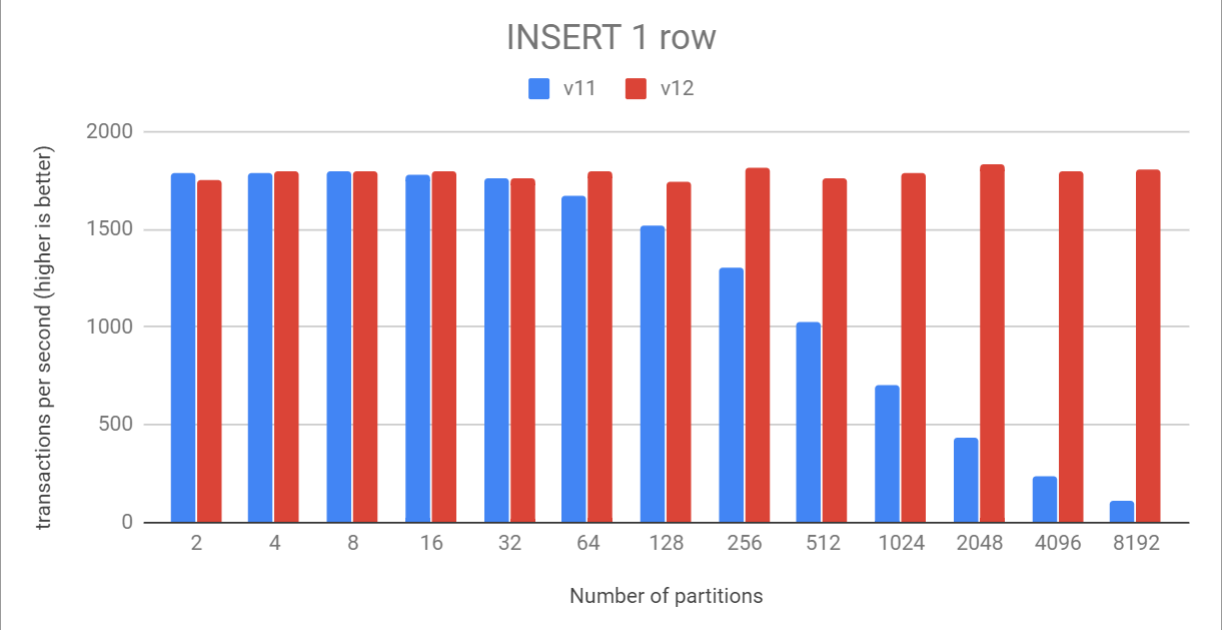
\includegraphics{insert-one-row.png}
\end{frame}
\begin{frame}
	\center
	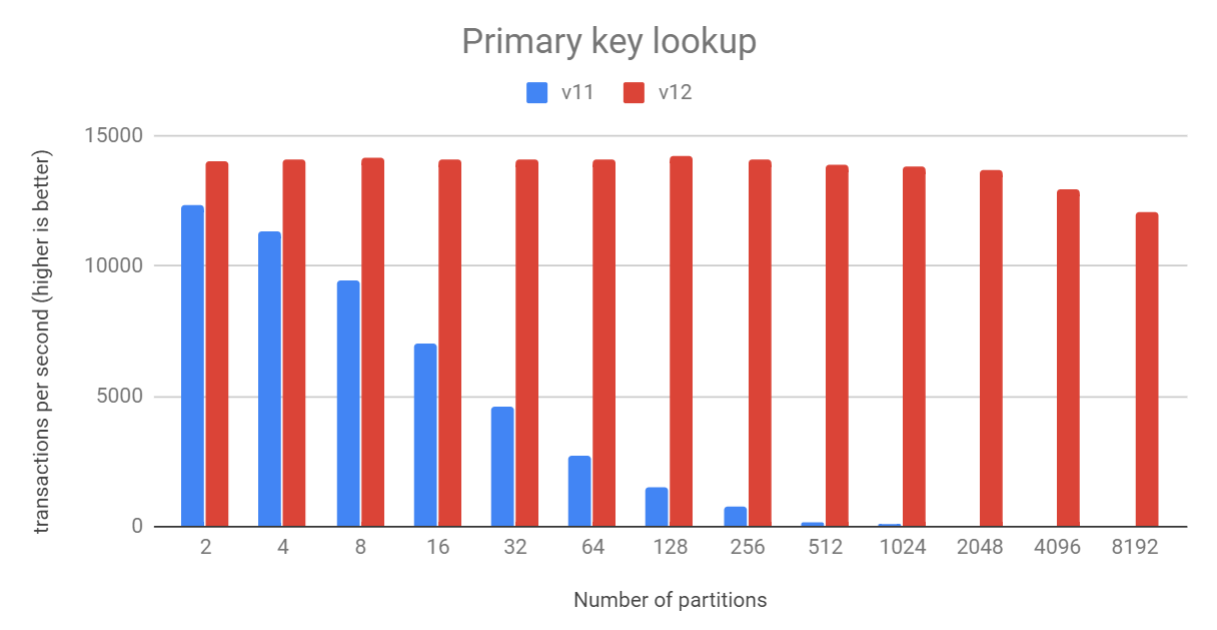
\includegraphics{pk-lookup.png}
\end{frame}
\begin{frame}
	\center
	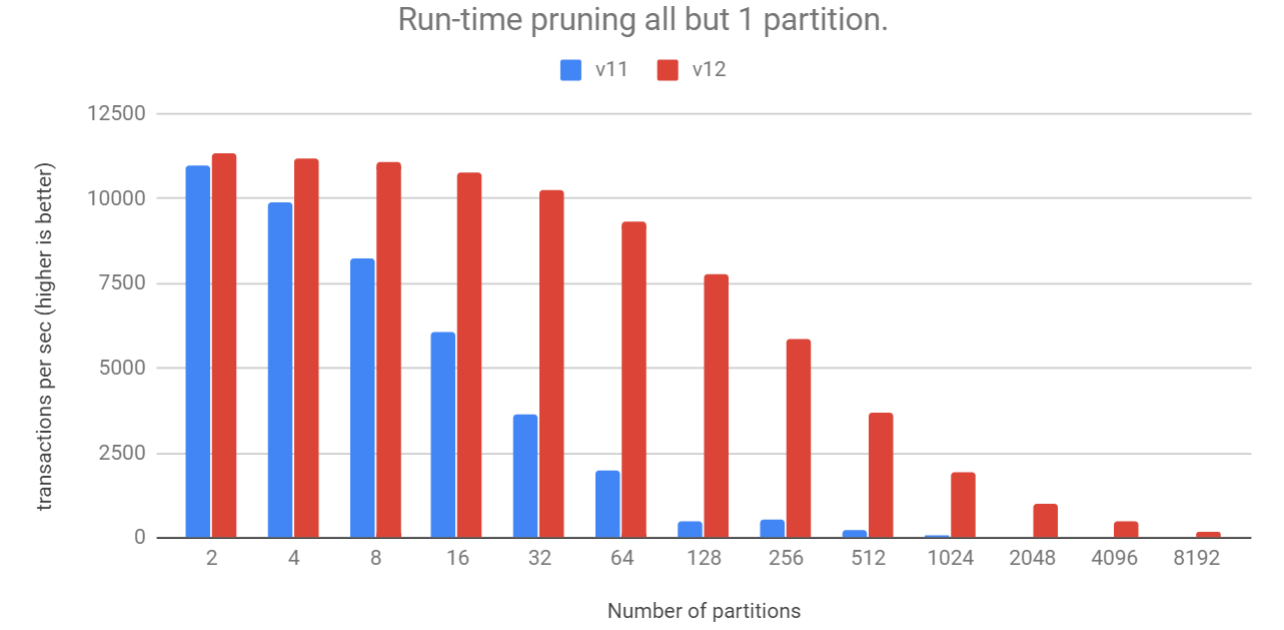
\includegraphics{runtime-prune.png}
\end{frame}
\begin{frame}
	\center
	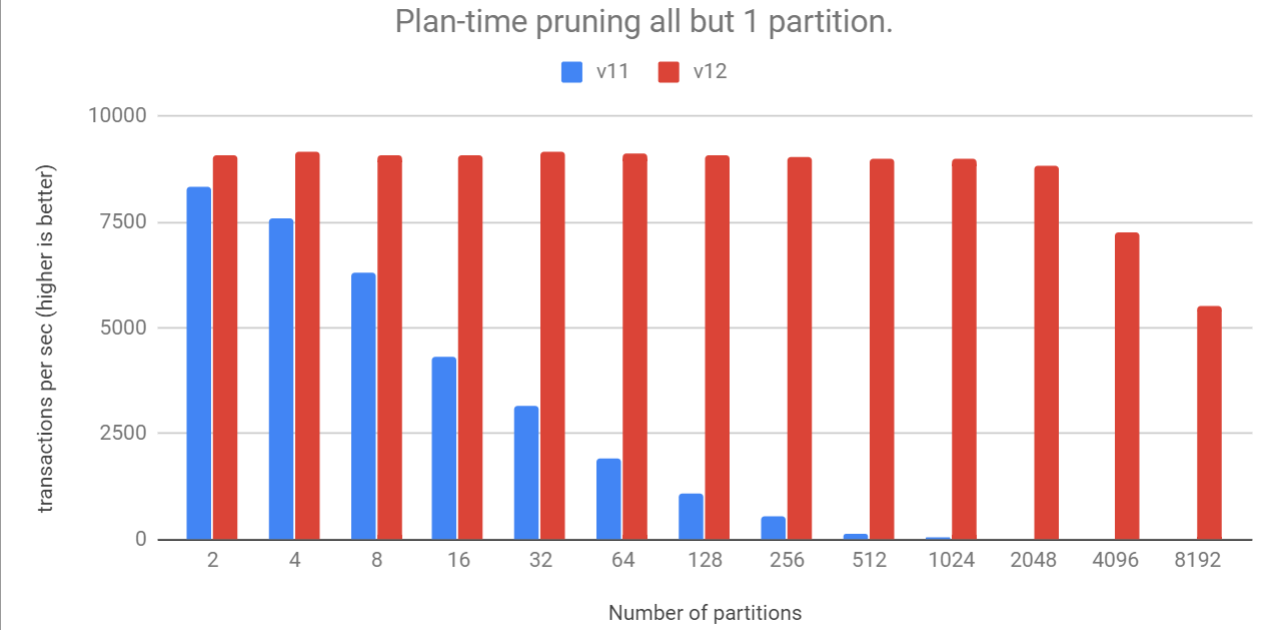
\includegraphics{plantime-prune.png}
\end{frame}

\section{Otros}
\begin{frame}
	\frametitle{Mantención (vacuum, analyze)}
	\begin{itemize}
		\item Mayoría de operaciones de mantención funcionan por partición
		\item Autovacuum se hace cargo en forma normal
		\item Única excepción: ANALYZE a la jerarquía completa
		\item En proceso para PostgreSQL 14
	\end{itemize}
\end{frame}

\begin{frame}[fragile]
	\frametitle{Replicación Lógica}

\begin{lstlisting}
CREATE PUBLICATION pub_clientes FOR TABLE clientes;

ALTER PUBLICATION pub_productos ADD TABLE productos;
\end{lstlisting}

\end{frame}

\begin{frame}
	\frametitle{Particionamiento: futuro cercano}

	\begin{itemize}
		\item REINDEX CONCURRENTLY
		\item CREATE INDEX CONCURRENTLY
		\item ALTER TABLE .. DETACH CONCURRENTLY
			\pause
		\item Autovacuum: autoanalyze
			\pause
		\item \texttt{ModifyTable} (UPDATE, DELETE)
	\end{itemize}
\end{frame}

\begin{frame}
	\frametitle{Particionamiento: futuro lejano}
	\begin{itemize}
		\item Índices globales
		\item Append/MergeAppend asíncrono (FDW)
		\item Mejoras para particiones tablas foráneas
	\end{itemize}
\end{frame}

\begin{frame}
	\frametitle{¿Preguntas?}

	\begin{center}
	\Large Agradezco su atención
	\end{center}
	\vskip 4cm
	
	\begin{itemize}
		\item \texttt{pgsql-es-ayuda@lists.postgresql.org}
		\item \texttt{info@2ndQuadrant.com}
	\end{itemize}
\end{frame}

\section{JOINs a nivel de partición}

\begin{frame}[fragile]
	\frametitle{Ejemplo para JOINs a nivel de partición}

  \footnotesize
  \begin{lstlisting}
CREATE TABLE orders (order_id int, client_id int) PARTITION BY RANGE (order_id);
CREATE TABLE orders_1000 PARTITION OF orders for values FROM (1) TO (1000);
CREATE TABLE orders_2000 PARTITION OF orders FOR VALUES FROM (1000) TO (2000);

CREATE TABLE order_items (order_id int, item_id int) PARTITION BY RANGE (order_id);
CREATE TABLE order_items_1000 PARTITION OF order_items for VALUES FROM (1) TO (1000);
CREATE TABLE order_items_2000 PARTITION OF order_items FOR VALUES FROM (1000) TO (2000);
  \end{lstlisting}

\end{frame}

\begin{frame}[fragile]
	\frametitle{Ejemplo sin JOINs a nivel de partición}

\begin{itemize} \item PostgreSQL 11 \end{itemize}
\footnotesize
  \begin{lstlisting}
SET enable_partitionwise_join TO off;
EXPLAIN (COSTS OFF)
  SELECT * FROM orders JOIN order_items USING (order_id)
  WHERE customer_id = 64;
  \end{lstlisting}
\end{frame}
\begin{frame}[fragile]
	\frametitle{Sin JOIN a nivel de partición}
	\begin{lstlisting}
 Hash Join
   Hash Cond: (order_items_1000.order_id = orders_1000.order_id)
   ->  Append
         ->  Seq Scan on order_items_1000
         ->  Seq Scan on order_items_2000
   ->  Hash
         ->  Append
               ->  Bitmap Heap Scan on orders_1000
                     Recheck Cond: (customer_id = 64)
                     ->  Bitmap Index Scan on orders_1000_customer_id_idx
                           Index Cond: (customer_id = 64)
               ->  Seq Scan on orders_2000
                     Filter: (customer_id = 64)
  \end{lstlisting}
\end{frame}

\begin{frame}[fragile]
	\frametitle{Activando JOIN a nivel de partición}

\scriptsize
  \begin{lstlisting}
 Append
   ->  Hash Join
         Hash Cond: (order_items_1000.order_id = orders_1000.order_id)
         ->  Seq Scan on order_items_1000
         ->  Hash
               ->  Bitmap Heap Scan on orders_1000
                     Recheck Cond: (customer_id = 64)
                     ->  Bitmap Index Scan on orders_1000_customer_id_idx
                           Index Cond: (customer_id = 64)
   ->  Nested Loop
         ->  Seq Scan on orders_2000
               Filter: (customer_id = 64)
         ->  Index Scan using order_items_2000_order_id_idx on order_items_2000
               Index Cond: (order_id = orders_2000.order_id)
  \end{lstlisting}

\end{frame}

\begin{frame}
	\frametitle{JOINs a nivel de partición: avanzado}

	\begin{itemize}
		\item PostgreSQL 13
		\item Las estrategias de partición ya no requieren ser idénticas
	\end{itemize}
\end{frame}

\section{Rehashing}

\begin{frame}[fragile]
	\frametitle{Rehashing: inicial}

  \begin{lstlisting}
CREATE TABLE clientes (
  cliente_id INTEGER, ...
) PARTITION BY HASH (cliente_id);

CREATE TABLE clientes_0 PARTITION OF clientes FOR VALUES WITH (MODULUS 3, REMAINDER 0);
CREATE TABLE clientes_1 PARTITION OF clientes FOR VALUES WITH (MODULUS 3, REMAINDER 1);

CREATE TABLE clientes_2 PARTITION OF clientes FOR VALUES WITH (MODULUS 6, REMAINDER 2);
CREATE TABLE clientes_5 PARTITION OF clientes FOR VALUES WITH (MODULUS 6, REMAINDER 5);
  \end{lstlisting}
\end{frame}

\begin{frame}[fragile]
	\frametitle{Rehashing: migración}
	\scriptsize
	\begin{lstlisting}
CREATE TABLE clientes_00 (LIKE clientes);
CREATE TABLE clientes_01 (LIKE clientes);

WITH moved AS (
  DELETE FROM clientes_0
    WHERE satisfies_hash_partition('clientes'::regclass, 6, 0, cliente_id)
    RETURNING *)
INSERT INTO clientes_00 SELECT * FROM moved;

WITH moved AS (
  DELETE FROM clientes_0
    WHERE satisfies_hash_partition('clientes'::regclass, 6, 3, cliente_id)
    RETURNING *)
INSERT INTO clientes_01 SELECT * FROM moved;
	\end{lstlisting}
\end{frame}

\end{document}

% :vim:ts=4:sw=4
